\documentclass[]{article}
\usepackage{lmodern}
\usepackage{amssymb,amsmath}
\usepackage{ifxetex,ifluatex}
\usepackage{fixltx2e} % provides \textsubscript
\ifnum 0\ifxetex 1\fi\ifluatex 1\fi=0 % if pdftex
  \usepackage[T1]{fontenc}
  \usepackage[utf8]{inputenc}
\else % if luatex or xelatex
  \ifxetex
    \usepackage{mathspec}
  \else
    \usepackage{fontspec}
  \fi
  \defaultfontfeatures{Ligatures=TeX,Scale=MatchLowercase}
\fi
% use upquote if available, for straight quotes in verbatim environments
\IfFileExists{upquote.sty}{\usepackage{upquote}}{}
% use microtype if available
\IfFileExists{microtype.sty}{%
\usepackage{microtype}
\UseMicrotypeSet[protrusion]{basicmath} % disable protrusion for tt fonts
}{}
\usepackage[margin=1in]{geometry}
\usepackage{hyperref}
\hypersetup{unicode=true,
            pdftitle={02\_Data\_Visualization},
            pdfauthor={Matt Dube},
            pdfborder={0 0 0},
            breaklinks=true}
\urlstyle{same}  % don't use monospace font for urls
\usepackage{color}
\usepackage{fancyvrb}
\newcommand{\VerbBar}{|}
\newcommand{\VERB}{\Verb[commandchars=\\\{\}]}
\DefineVerbatimEnvironment{Highlighting}{Verbatim}{commandchars=\\\{\}}
% Add ',fontsize=\small' for more characters per line
\usepackage{framed}
\definecolor{shadecolor}{RGB}{248,248,248}
\newenvironment{Shaded}{\begin{snugshade}}{\end{snugshade}}
\newcommand{\AlertTok}[1]{\textcolor[rgb]{0.94,0.16,0.16}{#1}}
\newcommand{\AnnotationTok}[1]{\textcolor[rgb]{0.56,0.35,0.01}{\textbf{\textit{#1}}}}
\newcommand{\AttributeTok}[1]{\textcolor[rgb]{0.77,0.63,0.00}{#1}}
\newcommand{\BaseNTok}[1]{\textcolor[rgb]{0.00,0.00,0.81}{#1}}
\newcommand{\BuiltInTok}[1]{#1}
\newcommand{\CharTok}[1]{\textcolor[rgb]{0.31,0.60,0.02}{#1}}
\newcommand{\CommentTok}[1]{\textcolor[rgb]{0.56,0.35,0.01}{\textit{#1}}}
\newcommand{\CommentVarTok}[1]{\textcolor[rgb]{0.56,0.35,0.01}{\textbf{\textit{#1}}}}
\newcommand{\ConstantTok}[1]{\textcolor[rgb]{0.00,0.00,0.00}{#1}}
\newcommand{\ControlFlowTok}[1]{\textcolor[rgb]{0.13,0.29,0.53}{\textbf{#1}}}
\newcommand{\DataTypeTok}[1]{\textcolor[rgb]{0.13,0.29,0.53}{#1}}
\newcommand{\DecValTok}[1]{\textcolor[rgb]{0.00,0.00,0.81}{#1}}
\newcommand{\DocumentationTok}[1]{\textcolor[rgb]{0.56,0.35,0.01}{\textbf{\textit{#1}}}}
\newcommand{\ErrorTok}[1]{\textcolor[rgb]{0.64,0.00,0.00}{\textbf{#1}}}
\newcommand{\ExtensionTok}[1]{#1}
\newcommand{\FloatTok}[1]{\textcolor[rgb]{0.00,0.00,0.81}{#1}}
\newcommand{\FunctionTok}[1]{\textcolor[rgb]{0.00,0.00,0.00}{#1}}
\newcommand{\ImportTok}[1]{#1}
\newcommand{\InformationTok}[1]{\textcolor[rgb]{0.56,0.35,0.01}{\textbf{\textit{#1}}}}
\newcommand{\KeywordTok}[1]{\textcolor[rgb]{0.13,0.29,0.53}{\textbf{#1}}}
\newcommand{\NormalTok}[1]{#1}
\newcommand{\OperatorTok}[1]{\textcolor[rgb]{0.81,0.36,0.00}{\textbf{#1}}}
\newcommand{\OtherTok}[1]{\textcolor[rgb]{0.56,0.35,0.01}{#1}}
\newcommand{\PreprocessorTok}[1]{\textcolor[rgb]{0.56,0.35,0.01}{\textit{#1}}}
\newcommand{\RegionMarkerTok}[1]{#1}
\newcommand{\SpecialCharTok}[1]{\textcolor[rgb]{0.00,0.00,0.00}{#1}}
\newcommand{\SpecialStringTok}[1]{\textcolor[rgb]{0.31,0.60,0.02}{#1}}
\newcommand{\StringTok}[1]{\textcolor[rgb]{0.31,0.60,0.02}{#1}}
\newcommand{\VariableTok}[1]{\textcolor[rgb]{0.00,0.00,0.00}{#1}}
\newcommand{\VerbatimStringTok}[1]{\textcolor[rgb]{0.31,0.60,0.02}{#1}}
\newcommand{\WarningTok}[1]{\textcolor[rgb]{0.56,0.35,0.01}{\textbf{\textit{#1}}}}
\usepackage{graphicx,grffile}
\makeatletter
\def\maxwidth{\ifdim\Gin@nat@width>\linewidth\linewidth\else\Gin@nat@width\fi}
\def\maxheight{\ifdim\Gin@nat@height>\textheight\textheight\else\Gin@nat@height\fi}
\makeatother
% Scale images if necessary, so that they will not overflow the page
% margins by default, and it is still possible to overwrite the defaults
% using explicit options in \includegraphics[width, height, ...]{}
\setkeys{Gin}{width=\maxwidth,height=\maxheight,keepaspectratio}
\IfFileExists{parskip.sty}{%
\usepackage{parskip}
}{% else
\setlength{\parindent}{0pt}
\setlength{\parskip}{6pt plus 2pt minus 1pt}
}
\setlength{\emergencystretch}{3em}  % prevent overfull lines
\providecommand{\tightlist}{%
  \setlength{\itemsep}{0pt}\setlength{\parskip}{0pt}}
\setcounter{secnumdepth}{0}
% Redefines (sub)paragraphs to behave more like sections
\ifx\paragraph\undefined\else
\let\oldparagraph\paragraph
\renewcommand{\paragraph}[1]{\oldparagraph{#1}\mbox{}}
\fi
\ifx\subparagraph\undefined\else
\let\oldsubparagraph\subparagraph
\renewcommand{\subparagraph}[1]{\oldsubparagraph{#1}\mbox{}}
\fi

%%% Use protect on footnotes to avoid problems with footnotes in titles
\let\rmarkdownfootnote\footnote%
\def\footnote{\protect\rmarkdownfootnote}

%%% Change title format to be more compact
\usepackage{titling}

% Create subtitle command for use in maketitle
\newcommand{\subtitle}[1]{
  \posttitle{
    \begin{center}\large#1\end{center}
    }
}

\setlength{\droptitle}{-2em}

  \title{02\_Data\_Visualization}
    \pretitle{\vspace{\droptitle}\centering\huge}
  \posttitle{\par}
    \author{Matt Dube}
    \preauthor{\centering\large\emph}
  \postauthor{\par}
      \predate{\centering\large\emph}
  \postdate{\par}
    \date{12/4/2018}


\begin{document}
\maketitle

{
\setcounter{tocdepth}{2}
\tableofcontents
}
Load libraries and set theme

\begin{Shaded}
\begin{Highlighting}[]
\KeywordTok{library}\NormalTok{(ggplot2)}
\KeywordTok{library}\NormalTok{(dplyr)}
\KeywordTok{library}\NormalTok{(ggthemes)}
\KeywordTok{library}\NormalTok{(here)}
\KeywordTok{library}\NormalTok{(readr)}
\KeywordTok{library}\NormalTok{(purrr)}
\KeywordTok{library}\NormalTok{(tidyr)}
\KeywordTok{library}\NormalTok{(vcd)}
\KeywordTok{library}\NormalTok{(corrplot)}
\end{Highlighting}
\end{Shaded}

\begin{Shaded}
\begin{Highlighting}[]
\KeywordTok{theme_set}\NormalTok{(}\KeywordTok{theme_light}\NormalTok{())}
\end{Highlighting}
\end{Shaded}

Load data

\begin{Shaded}
\begin{Highlighting}[]
\NormalTok{customer <-}\StringTok{ }\KeywordTok{read_csv}\NormalTok{(}\KeywordTok{here}\NormalTok{(}\StringTok{"00_Data/raw"}\NormalTok{, }\StringTok{"WA_Fn-UseC_-Telco-Customer-Churn.csv"}\NormalTok{))}
\end{Highlighting}
\end{Shaded}

Functions to assist with plotting

\begin{Shaded}
\begin{Highlighting}[]
\NormalTok{plotNumData <-}\StringTok{ }\ControlFlowTok{function}\NormalTok{(varList, inputData) \{}
    \KeywordTok{gather}\NormalTok{(}\DataTypeTok{data=}\NormalTok{inputData, varList, }\DataTypeTok{key =} \StringTok{"var"}\NormalTok{, }\DataTypeTok{value =} \StringTok{"value"}\NormalTok{) }\OperatorTok
\StringTok{        }\KeywordTok{ggplot}\NormalTok{(}\KeywordTok{aes}\NormalTok{(}\DataTypeTok{x=}\NormalTok{Churn, }\DataTypeTok{y=}\NormalTok{value, }\DataTypeTok{fill=}\NormalTok{Churn)) }\OperatorTok{+}
\StringTok{        }\KeywordTok{geom_boxplot}\NormalTok{() }\OperatorTok{+}
\StringTok{        }\KeywordTok{facet_wrap}\NormalTok{(}\OperatorTok{~}\StringTok{ }\NormalTok{var, }\DataTypeTok{scales =} \StringTok{"free"}\NormalTok{) }\OperatorTok{+}
\StringTok{        }\KeywordTok{scale_fill_brewer}\NormalTok{(}\DataTypeTok{palette =} \StringTok{"Paired"}\NormalTok{)}
\NormalTok{\}}

\NormalTok{plotCharData <-}\StringTok{ }\ControlFlowTok{function}\NormalTok{(varList, inputData) \{}
    \KeywordTok{gather}\NormalTok{(}\DataTypeTok{data=}\NormalTok{inputData, varList, }\DataTypeTok{key =} \StringTok{"var"}\NormalTok{, }\DataTypeTok{value =} \StringTok{"value"}\NormalTok{) }\OperatorTok
\StringTok{        }\KeywordTok{ggplot}\NormalTok{(}\KeywordTok{aes}\NormalTok{(}\DataTypeTok{x=}\NormalTok{value, }\DataTypeTok{fill=}\NormalTok{Churn)) }\OperatorTok{+}
\StringTok{        }\KeywordTok{geom_bar}\NormalTok{() }\OperatorTok{+}
\StringTok{        }\KeywordTok{coord_flip}\NormalTok{() }\OperatorTok{+}
\StringTok{        }\KeywordTok{facet_wrap}\NormalTok{(}\OperatorTok{~}\StringTok{ }\NormalTok{var, }\DataTypeTok{scales=}\StringTok{"free"}\NormalTok{) }\OperatorTok{+}
\StringTok{        }\KeywordTok{scale_fill_brewer}\NormalTok{(}\DataTypeTok{palette =} \StringTok{"Paired"}\NormalTok{)}
\NormalTok{\}}

\NormalTok{plotHistograms <-}\StringTok{ }\ControlFlowTok{function}\NormalTok{(varList, inputData) \{}
    \KeywordTok{gather}\NormalTok{(}\DataTypeTok{data=}\NormalTok{inputData, varList, }\DataTypeTok{key =} \StringTok{"var"}\NormalTok{, }\DataTypeTok{value =} \StringTok{"value"}\NormalTok{) }\OperatorTok
\StringTok{        }\KeywordTok{ggplot}\NormalTok{(}\KeywordTok{aes}\NormalTok{(}\DataTypeTok{x=}\NormalTok{value, }\DataTypeTok{fill=}\NormalTok{Churn)) }\OperatorTok{+}
\StringTok{        }\KeywordTok{geom_histogram}\NormalTok{() }\OperatorTok{+}
\StringTok{        }\KeywordTok{facet_wrap}\NormalTok{(}\OperatorTok{~}\StringTok{ }\NormalTok{var, }\DataTypeTok{scales =} \StringTok{"free"}\NormalTok{, }\DataTypeTok{ncol =} \DecValTok{2}\NormalTok{) }\OperatorTok{+}
\StringTok{        }\KeywordTok{scale_fill_brewer}\NormalTok{(}\DataTypeTok{palette =} \StringTok{"Paired"}\NormalTok{)}
\NormalTok{\}}
\end{Highlighting}
\end{Shaded}

Boxplots of numeric features

\begin{Shaded}
\begin{Highlighting}[]
\NormalTok{numVarToPlot <-}\StringTok{ }\KeywordTok{c}\NormalTok{(}\StringTok{"tenure"}\NormalTok{, }\StringTok{"MonthlyCharges"}\NormalTok{, }\StringTok{"TotalCharges"}\NormalTok{)}
\KeywordTok{plotNumData}\NormalTok{(numVarToPlot, customer)}
\end{Highlighting}
\end{Shaded}

\begin{verbatim}
## Warning: Removed 11 rows containing non-finite values (stat_boxplot).
\end{verbatim}

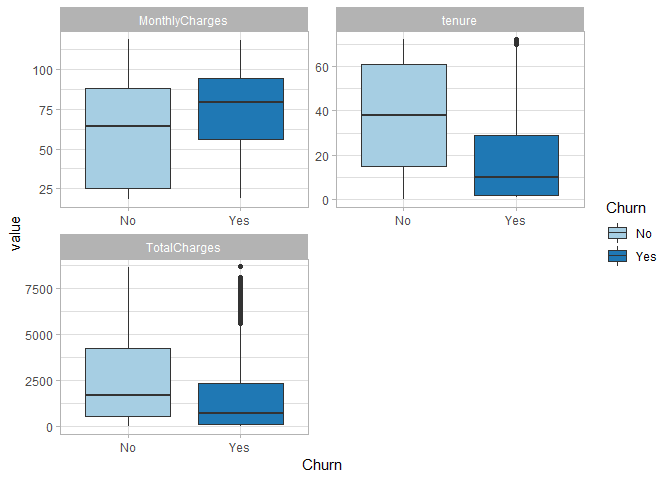
\includegraphics{02_Data_Visualization_files/figure-latex/unnamed-chunk-5-1.pdf}
Histograms of numeric features

\begin{Shaded}
\begin{Highlighting}[]
\KeywordTok{plotHistograms}\NormalTok{(numVarToPlot, customer)}
\end{Highlighting}
\end{Shaded}

\begin{verbatim}
## `stat_bin()` using `bins = 30`. Pick better value with `binwidth`.
\end{verbatim}

\begin{verbatim}
## Warning: Removed 11 rows containing non-finite values (stat_bin).
\end{verbatim}

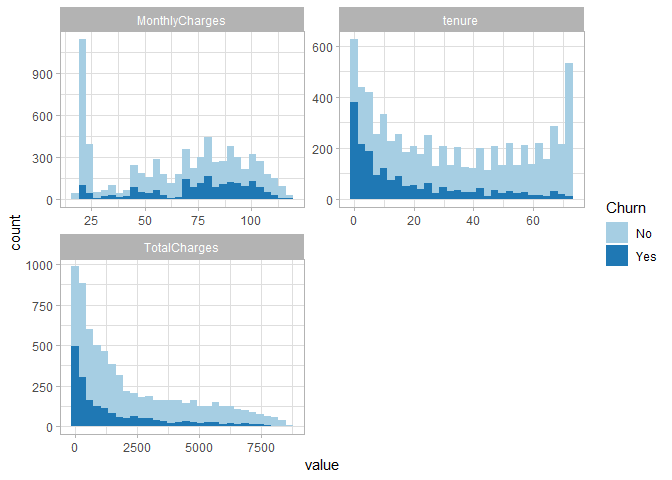
\includegraphics{02_Data_Visualization_files/figure-latex/unnamed-chunk-6-1.pdf}

Notes on numeric features:

\begin{itemize}
\tightlist
\item
  customers with smaller tenures and higher monthly charges are more
  likely to churn.
\item
  there are a few long tenured customers who have churned, and appear as
  outliers in the boxplot.
\item
  total charges has a few potential outliers as well that need to be
  examined.
\end{itemize}

Bar plots of character features

\begin{Shaded}
\begin{Highlighting}[]
\NormalTok{varToPlot <-}\StringTok{ }\KeywordTok{c}\NormalTok{(}\StringTok{"gender"}\NormalTok{, }\StringTok{"Partner"}\NormalTok{, }\StringTok{"Dependents"}\NormalTok{, }\StringTok{"PhoneService"}\NormalTok{)}
\KeywordTok{plotCharData}\NormalTok{(varToPlot, customer)}
\end{Highlighting}
\end{Shaded}

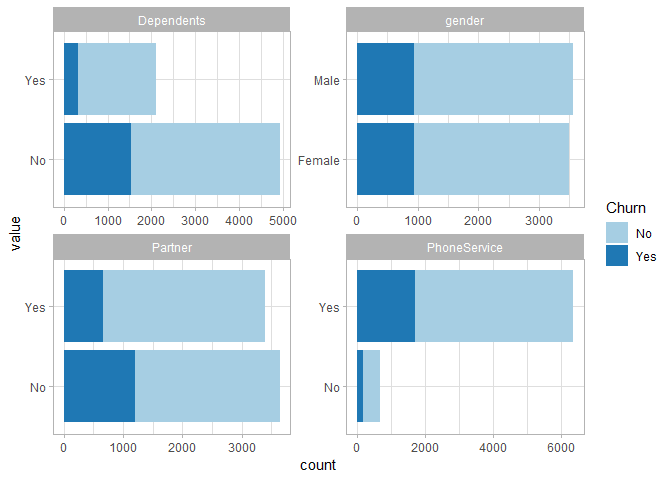
\includegraphics{02_Data_Visualization_files/figure-latex/unnamed-chunk-7-1.pdf}

\begin{Shaded}
\begin{Highlighting}[]
\NormalTok{varToPlot <-}\StringTok{ }\KeywordTok{c}\NormalTok{(}\StringTok{"MultipleLines"}\NormalTok{, }\StringTok{"InternetService"}\NormalTok{, }\StringTok{"OnlineSecurity"}\NormalTok{, }\StringTok{"OnlineBackup"}\NormalTok{)}
\KeywordTok{plotCharData}\NormalTok{(varToPlot, customer)}
\end{Highlighting}
\end{Shaded}

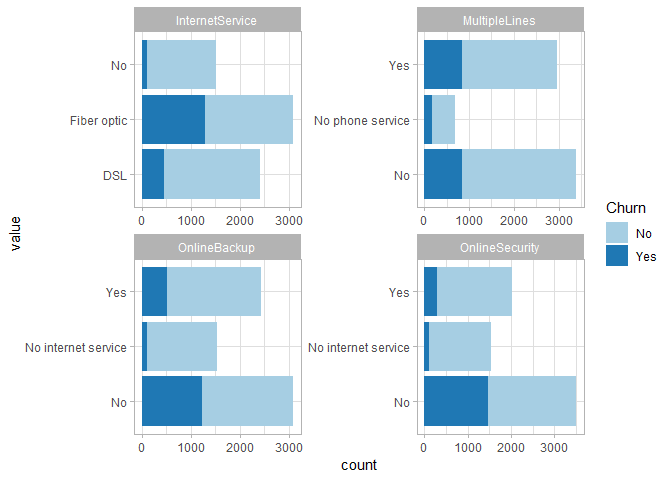
\includegraphics{02_Data_Visualization_files/figure-latex/unnamed-chunk-8-1.pdf}

\begin{Shaded}
\begin{Highlighting}[]
\NormalTok{varToPlot <-}\StringTok{ }\KeywordTok{c}\NormalTok{(}\StringTok{"MultipleLines"}\NormalTok{, }\StringTok{"InternetService"}\NormalTok{, }\StringTok{"OnlineSecurity"}\NormalTok{, }\StringTok{"OnlineBackup"}\NormalTok{)}
\KeywordTok{plotCharData}\NormalTok{(varToPlot, customer)}
\end{Highlighting}
\end{Shaded}

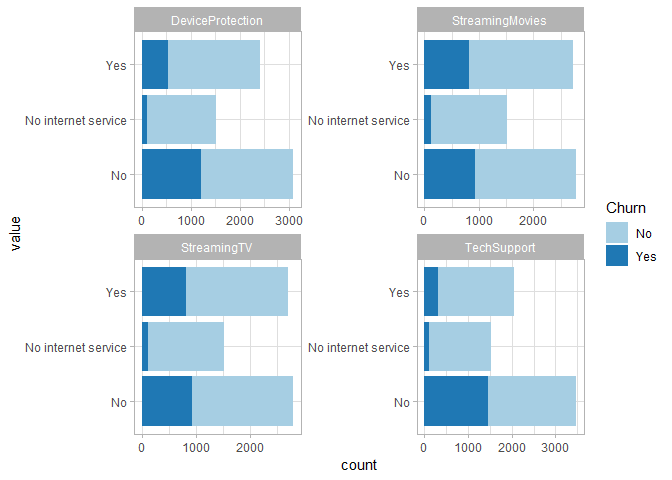
\includegraphics{02_Data_Visualization_files/figure-latex/unnamed-chunk-9-1.pdf}

Review correlation between TotalCharges and MonthlyCharges.

\begin{Shaded}
\begin{Highlighting}[]
\NormalTok{cust_numeric <-}\StringTok{ }
\StringTok{    }\NormalTok{customer }\OperatorTok
\StringTok{    }\KeywordTok{select}\NormalTok{(}\OperatorTok{-}\NormalTok{SeniorCitizen) }\OperatorTok
\StringTok{    }\KeywordTok{keep}\NormalTok{(is.numeric)}
\end{Highlighting}
\end{Shaded}

\begin{Shaded}
\begin{Highlighting}[]
\NormalTok{M <-}\StringTok{ }\KeywordTok{cor}\NormalTok{(cust_numeric,}\DataTypeTok{use=}\StringTok{"complete.obs"}\NormalTok{)}
\end{Highlighting}
\end{Shaded}

\begin{Shaded}
\begin{Highlighting}[]
\KeywordTok{corrplot}\NormalTok{(M, }\DataTypeTok{method=}\StringTok{"number"}\NormalTok{, }\DataTypeTok{type=}\StringTok{"lower"}\NormalTok{)}
\end{Highlighting}
\end{Shaded}

\includegraphics{02_Data_Visualization_files/figure-latex/unnamed-chunk-12-1.pdf}


\end{document}
